\documentclass{article}
% translate with >> pdflatex -shell-escape <file>

% This file is used as unit test for pgfplots, copyright by Christian Feuersaenger.
% 
% See
%   http://pgfplots.sourceforge.net/pgfplots.pdf
% for pgfplots.
%
% Any required input files (for <plot table> or <plot file> or the table package) can be downloaded
% at
% http://www.ctan.org/tex-archive/graphics/pgf/contrib/pgfplots/doc/latex/
% and
% http://www.ctan.org/tex-archive/graphics/pgf/contrib/pgfplots/doc/latex/plotdata/

\usepackage{pgfplots}
\pgfplotsset{compat=newest}

\pagestyle{empty}

\begin{document}
\section{Scale vs. Datascale trafo}
All should have the same size; especially the same height.
This tests the data scale transformation and rounding inaccuracies during the computation of $x$~and~$y$ unit vectors,
\[ x = \frac{W}{T(\bar x) - T(\underline x)}. \]
The larger $x$, the higher the scaling accuracy. Large $x$ means small $T(\bar x) - T(\underline x)$ (relative to width~$W$). But this implies low accuracy for the input data! And nobody wants inaccurate plots.

The datascale transformation~$T$ is set up such that $O(W) = O(x)$, but I am not sure if I need to adjust some parameters. Some parameters lead to inaccurate~$x$ and~$y$ vectors, such that axis sizes are \emph{not} the same although $W$~and~$H$ (width and height) are the same.

\noindent
{\pgfplotsset{every picture/.append style={baseline}}
\pgfplotsset{every axis/.append style={width=3cm,scale only axis,ytick=\empty,cycle list=blue}}%
\def\TESTPLOTS{%
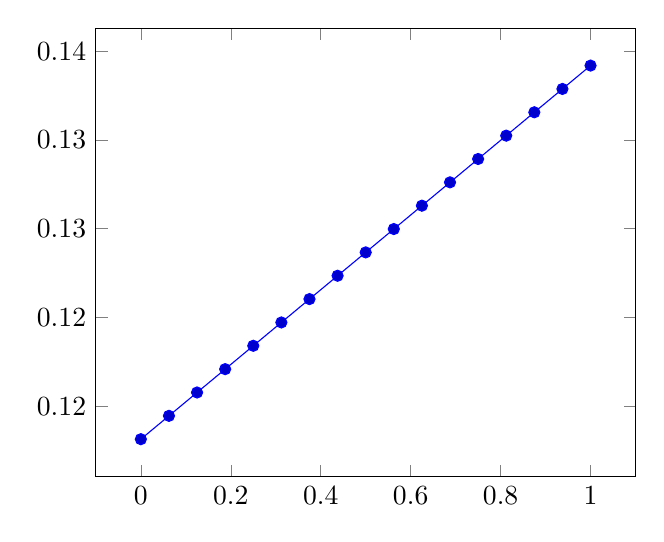
\begin{tikzpicture}%
\begin{axis}
\addplot plot coordinates {
	(0.000000,	0.113142)
	(0.062500,	0.114457)
	(0.125000,	0.115773)
	(0.187500,	0.117088)
	(0.250000,	0.118404)
	(0.312500,	0.119719)
	(0.375000,	0.121035)
	(0.437500,	0.122350)
	(0.500000,	0.123666)
	(0.562500,	0.124981)
	(0.625000,	0.126297)
	(0.687500,	0.127612)
	(0.750000,	0.128928)
	(0.812500,	0.130243)
	(0.875000,	0.131559)
	(0.937500,	0.132874)
	(1.000000,	0.134190)
};
\end{axis}
\end{tikzpicture}%
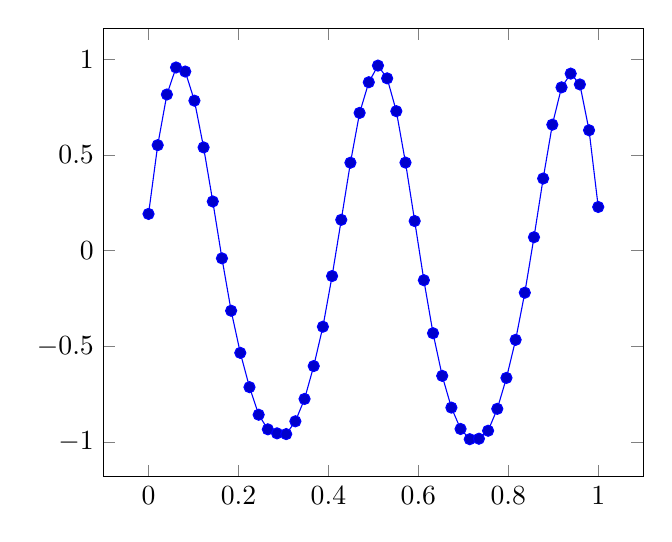
\begin{tikzpicture}%
\begin{axis}
\addplot plot coordinates {
	(0.000000,	0.192392)
	(0.020408,	0.551660)
	(0.040816,	0.816371)
	(0.061224,	0.957528)
	(0.081633,	0.936301)
	(0.102041,	0.784097)
	(0.122449,	0.539922)
	(0.142857,	0.257432)
	(0.163265,	-0.039651)
	(0.183673,	-0.313379)
	(0.204082,	-0.533386)
	(0.224490,	-0.712582)
	(0.244898,	-0.856655)
	(0.265306,	-0.932880)
	(0.285714,	-0.953862)
	(0.306122,	-0.957749)
	(0.326531,	-0.890993)
	(0.346939,	-0.774152)
	(0.367347,	-0.602360)
	(0.387755,	-0.396801)
	(0.408163,	-0.132261)
	(0.428571,	0.161664)
	(0.448980,	0.460018)
	(0.469388,	0.720198)
	(0.489796,	0.880398)
	(0.510204,	0.967384)
	(0.530612,	0.900632)
	(0.551020,	0.729232)
	(0.571429,	0.460479)
	(0.591837,	0.155311)
	(0.612245,	-0.153827)
	(0.632653,	-0.430787)
	(0.653061,	-0.653561)
	(0.673469,	-0.819444)
	(0.693878,	-0.931060)
	(0.714286,	-0.984394)
	(0.734694,	-0.981970)
	(0.755102,	-0.940272)
	(0.775510,	-0.825804)
	(0.795918,	-0.664138)
	(0.816327,	-0.465371)
	(0.836735,	-0.219185)
	(0.857143,	0.070697)
	(0.877551,	0.377456)
	(0.897959,	0.658660)
	(0.918367,	0.853564)
	(0.938776,	0.925472)
	(0.959184,	0.868936)
	(0.979592,	0.629528)
	(1.000000,	0.228732)
};
\end{axis}
\end{tikzpicture}%
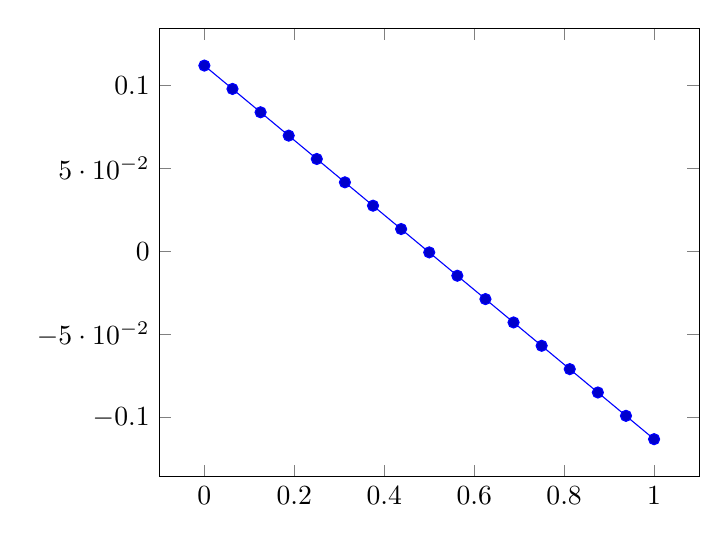
\begin{tikzpicture}%
\begin{axis}

\addplot plot coordinates {
	(0.000000,	0.112104)
	(0.062500,	0.098029)
	(0.125000,	0.083954)
	(0.187500,	0.069879)
	(0.250000,	0.055804)
	(0.312500,	0.041729)
	(0.375000,	0.027654)
	(0.437500,	0.013579)
	(0.500000,	-0.000496)
	(0.562500,	-0.014571)
	(0.625000,	-0.028646)
	(0.687500,	-0.042722)
	(0.750000,	-0.056797)
	(0.812500,	-0.070872)
	(0.875000,	-0.084947)
	(0.937500,	-0.099022)
	(1.000000,	-0.113097)
};
\end{axis}
\end{tikzpicture}%
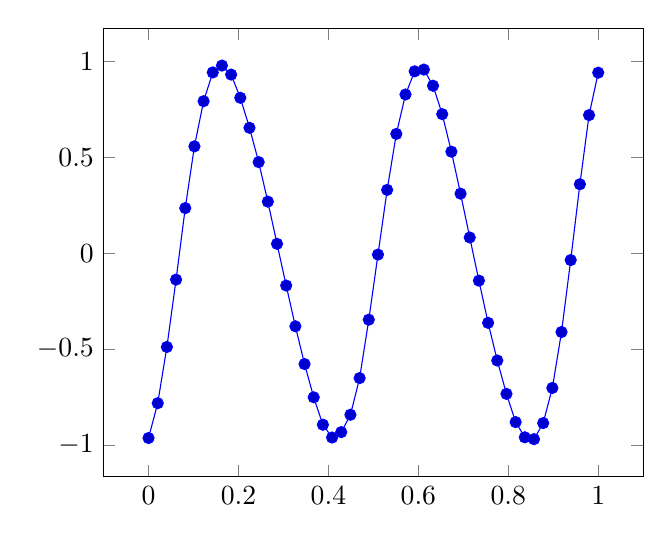
\begin{tikzpicture}%
\begin{axis}
\addplot plot coordinates {
	(0.000000,	-0.963159)
	(0.020408,	-0.781664)
	(0.040816,	-0.488585)
	(0.061224,	-0.137738)
	(0.081633,	0.234861)
	(0.102041,	0.556489)
	(0.122449,	0.791942)
	(0.142857,	0.941856)
	(0.163265,	0.977486)
	(0.183673,	0.930499)
	(0.204082,	0.809581)
	(0.224490,	0.653308)
	(0.244898,	0.474588)
	(0.265306,	0.268631)
	(0.285714,	0.048692)
	(0.306122,	-0.168568)
	(0.326531,	-0.380963)
	(0.346939,	-0.577633)
	(0.367347,	-0.751043)
	(0.387755,	-0.893755)
	(0.408163,	-0.960465)
	(0.428571,	-0.932380)
	(0.448980,	-0.841830)
	(0.469388,	-0.650880)
	(0.489796,	-0.346509)
	(0.510204,	-0.007265)
	(0.530612,	0.329744)
	(0.551020,	0.621489)
	(0.571429,	0.826905)
	(0.591837,	0.947602)
	(0.612245,	0.956706)
	(0.632653,	0.872426)
	(0.653061,	0.724325)
	(0.673469,	0.528915)
	(0.693878,	0.310032)
	(0.714286,	0.081807)
	(0.734694,	-0.143046)
	(0.755102,	-0.363063)
	(0.775510,	-0.559141)
	(0.795918,	-0.733031)
	(0.816327,	-0.880063)
	(0.836735,	-0.959350)
	(0.857143,	-0.968957)
	(0.877551,	-0.885145)
	(0.897959,	-0.702171)
	(0.918367,	-0.410704)
	(0.938776,	-0.035900)
	(0.959184,	0.359062)
	(0.979592,	0.719407)
	(1.000000,	0.940563)
};
\end{axis}
\end{tikzpicture}%
}%
\TESTPLOTS

once more again without `scale only axis':
\pgfplotsset{every axis/.append style={scale only axis=false}}%

\TESTPLOTS
}
\end{document}
